\section{Visualiser Tool}\label{sec:visualiser}
The Visualiser is a tool written in Python and JavaScript, created by Peter Gjøl Jensen. The tool was created
to aid in the visualisation of \gls{manet} topologies and works by importing a log file with \acrshort{gps}
coordinates and timestamps for a series of nodes. Using the tool, it is possible to visualise the position and
movement for all nodes in a network. A snippet of a \acrshort{gps} log can be seen below. Each line consists
of the identifier of the node, the latitude and longitude coordinates for the node, and the timestamp for the
coordinates in milliseconds. We found the tool to be able to handle visualisations up to around 100 nodes.
%
\begin{verbatim}
#id,lat,lon,timestamp
64,14.629879,121.096137,158980000.000000
64,14.629874,121.096132,159000000.000000
64,14.629878,121.096128,159020000.000000
64,14.629890,121.096143,159040000.000000
64,14.629892,121.096142,159060000.000000
64,14.629896,121.096141,159080000.000000
64,14.629893,121.096164,159100000.000000
64,14.629947,121.096083,159120000.000000
64,14.630107,121.095976,159140000.000000
64,14.630283,121.095885,159160000.000000
64,14.630525,121.095786,159180000.000000
\end{verbatim}

\begin{figure}[H]
    \centering
    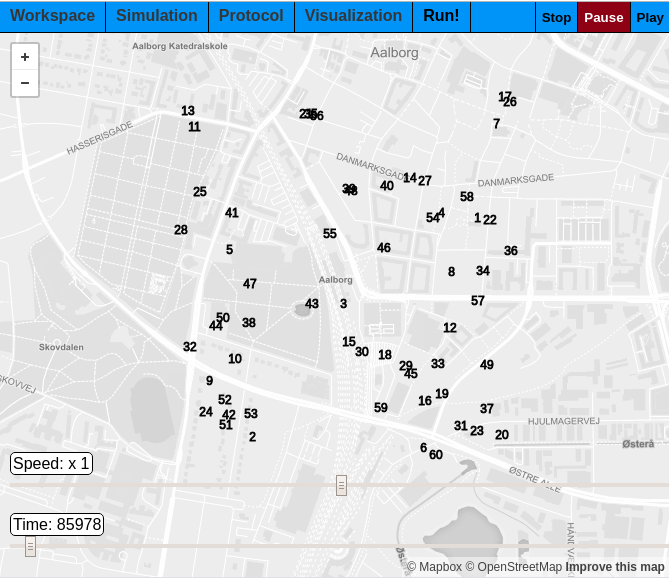
\includegraphics[width=.8\textwidth]{figures/visualiser/gpslog.png}
    \caption{A visualised \acrshort{gps} log.}
    \label{figure:gpslogvisualised}
\end{figure}

\autoref{figure:gpslogvisualised} shows a screen-shot from the Visualiser, with a \acrshort{gps} log loaded.
When a \acrshort{gps} log is loaded, the Visualiser can be started by pressing the \doublequote{Play} button,
or the \doublequote{space} key. The speed of the visualisation can be controlled with the \doublequote{Speed}
slider in the bottom, and the current time of the visualisation can be controlled with the \doublequote{Time}
slider.

\subsection{Extensions}
We propose three extensions to the visualiser tool. The first is to visualise the link between nodes using an
annotated version of the \acrshort{gps} log, where each line is annotated with the \gls{rssi} of a link
between nodes in the log, as shown below. In the annotated log, each link for a given node, to another node,
is annotated, after the timestamp, with the identifier of the other node, and the \gls{rssi} between them.
\autoref{figure:gpslogrssivisualised} shows an example of a very connected
network where links between nodes are visualised by a colour gradient, where a link with a yellow colour has a
better \gls{rssi} than a link with a red colour. It is possible to print the \gls{rssi} value for the links as
well.
%
\begin{verbatim}
#id,lat,lon,timestamp,id1,rssi1,id2,rssi2,id3,rssi3, ...
65,14.630107,121.096749,157820000.000000,67,-56,69,-70,71,-13, ...
65,14.630129,121.096905,157840000.000000,67,-58,69,-61,73,-65, ...
65,14.630189,121.097116,157860000.000000,67,-55,69,-54,73,-71, ...
65,14.630318,121.097294,157880000.000000,67,-65,69,-66,71,-13, ...
65,14.630330,121.097545,157900000.000000,67,-79,69,-48,73,-79, ...
65,14.630358,121.097725,157920000.000000,67,-85,69,-66,71,-28, ...
65,14.630243,121.097900,157940000.000000,69,-84,71,-35,83,-67, ...
65,14.630082,121.098037,157960000.000000,71,-45,83,-70,89,-43, ...
65,14.629960,121.098165,157980000.000000,71,-20,83,-75,89,-38, ...
65,14.629729,121.098192,158000000.000000,83,-81,89,-42,97,-80, ...
\end{verbatim}

The second extension is to be able to replay the communication between nodes when simulating a protocol. This
log is generated by the Coordinator (introduced in \autoref{sec:coordinator}), and a line is added whenever a
packet is either dropped or received during transmission. Each line states whether the packet was received
or dropped, the identifier of the transmitter and receiver, the number of bytes sent, the \gls{rssi} for the
transmission, the probability for packet error, that decided whether the packet was dropped or not, the
interfering power and the number of interfering transmitters (if any), and finally, the start and end time of
the transmission. With this log, it is possible to visualise any transmissions by drawing a unidirectional
arrow from the transmitter to the receiver, within the time interval of the transmission.
%
\begin{verbatim}
#received,tx_id,rx_id,bytes,rssi,pep,int_power,ints,tx_start,tx_end
recv,1,2,2,-102.419,5.74662e-05,0,0,2233,2692
recv,1,5,2,-102.419,5.7577e-05,0,0,2233,2692
drop,1,6,2,-110.697,0.494838,0,0,2233,2692
drop,1,6,24,-110.697,0.999724,0,0,12692,18209
recv,1,5,24,-102.419,0.000690706,0,0,12692,18209
recv,1,2,24,-102.419,0.000689376,0,0,12692,18209
recv,1,2,2,-102.419,5.74662e-05,0,0,32002048,32002507
recv,1,5,24,-102.419,0.000690706,0,0,32012507,32018024
recv,1,2,24,-102.419,0.000689376,0,0,32012507,32018024
\end{verbatim}

\begin{figure}[H]
    \centering
    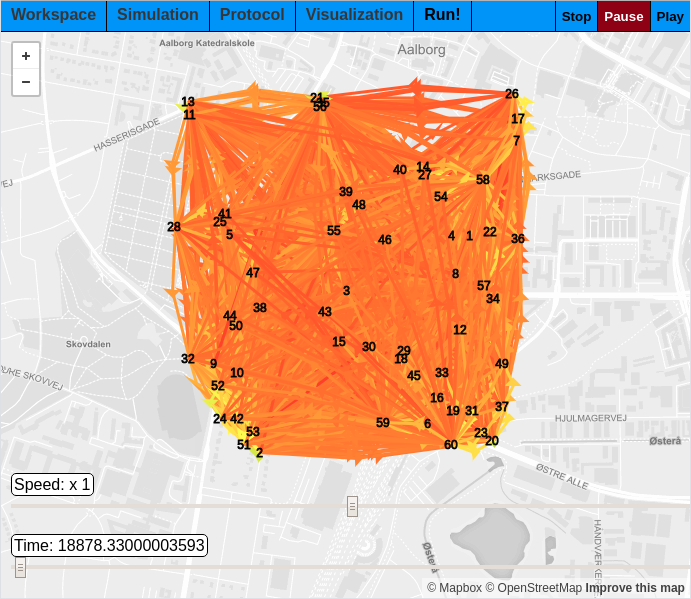
\includegraphics[width=.8\textwidth]{figures/visualiser/gpslog+rssi.png}
    \caption{A visualised \acrshort{gps} log with coloured links, based on \gls{rssi}.}
    \label{figure:gpslogrssivisualised}
\end{figure}
%

The third, and final, extension is to replay state changes of a protocol. When simulating a protocol like the
\gls{lmac} protocol (introduced in \autoref{sec:lmacc}), where each node proceeds through a number of states,
we log each of the state changes, as shown below, and can replay these state changes in the Visualiser.
%
\begin{verbatim}
#timestamp,id,state
0,10,i
0,1,i
0,9,i
800.009,1,0
800.002,2,w
5600,2,d
800.002,5,w
4800,5,d
5600.01,5,5
6400.01,2,6
6400,6,w
8800,6,d
\end{verbatim}

A visualised example of the second and third extension for an execution of the \gls{lmac} protocol can be
found in \autoref{fig:lmac-visualisation} in \autoref{sec:lmacc}, and in \autoref{figure:comproclogs}.

\begin{figure}[H]
    \centering
    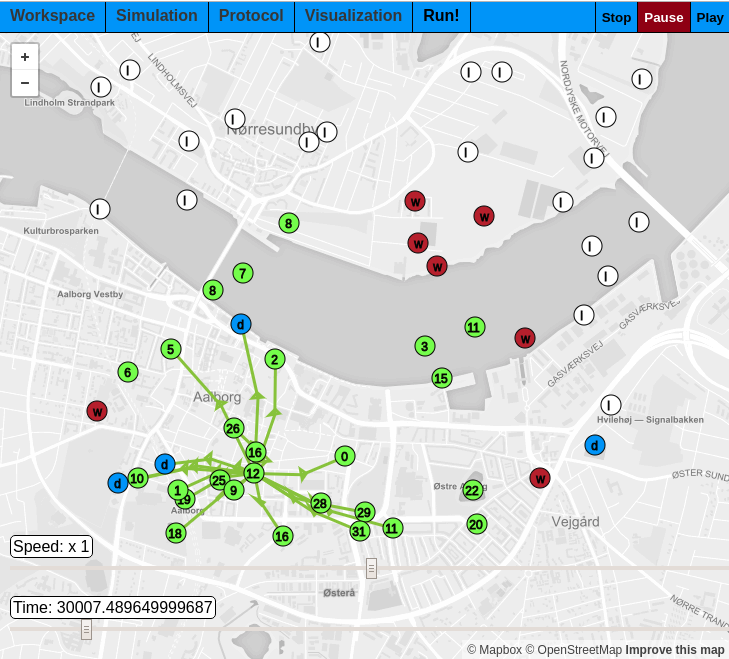
\includegraphics[width=.8\textwidth]{figures/visualiser/frontpage-visualisation.png}
    \caption{Communication and protocol logs visualised.}
    \label{figure:comproclogs}
\end{figure}

%\todo[inline]{introduce}
%\todo[inline]{why}
%\todo[inline]{screenshots and short description of what it can do}

The complete source code for the Visualiser tool can be found on GitHub:

{\small \url{https://github.com/Joklost/manet-simulations/tree/master/tools/visualiser}}
%